\documentclass{standalone}
\usepackage[dvipsnames]{xcolor}
\usepackage{tikz}

\usetikzlibrary{calc}

\tikzset{
    chat/.style={
        draw,
        rounded corners=5pt,
        minimum width=5cm,
        % minimum height=2cm,
        text width=3in,
        fill=gray!20
    },
    chatheader/.style={
        anchor=north west,
        font=\bfseries
    },
    chatline/.style={
        anchor=north west,
        text width=3in,
        font=\sffamily
    },
    chatlineother/.style={
        draw,
        color=RoyalBlue,
        rounded corners=5pt,
        anchor=south east,
        fill=RoyalBlue!20,
        text width=2in
    }
}

\begin{document}

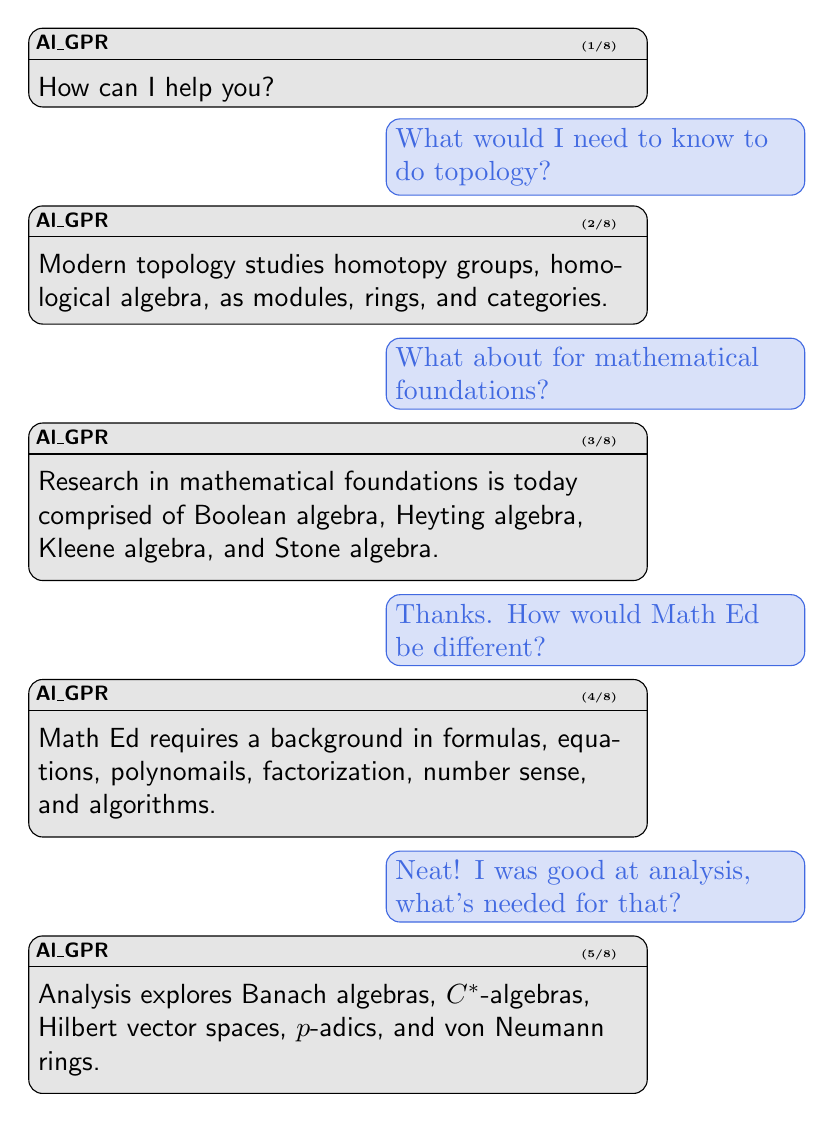
\begin{tikzpicture}

    \node (C1) [chat,minimum height=1cm] {};
    \node[chatheader,scale=0.75] at (C1.north west) {\textsf{Al\_GPR}\hspace{8cm}{\tiny (1/8)}};
    \draw ($(C1.north west) + (0,-0.4)$) -- ($(C1.north east) + (0,-0.4)$);
    \node[chatline] at ($(C1.north west) + (0,-0.5)$) {How can I help you?};

    %% Q1: Topology
    \node (Q1) [chatlineother] at ($(C1.south east) + (2cm,-1.12cm)$) {What would 
    I need to know to do topology?};

    \node (C2) [chat,minimum height=1.5cm] 
        at ($(C1.south)+(0,-2cm)$) {};
    \node[chatheader,scale=0.75] at (C2.north west) {\textsf{Al\_GPR}\hspace{8cm}{\tiny (2/8)}};
    \draw ($(C2.north west) + (0,-0.4)$) -- ($(C2.north east) + (0,-0.4)$);
    \node[chatline] at ($(C2.north west) + (0,-0.5)$) {Modern topology studies homotopy groups, homological algebra, as modules, rings, and categories.};

    %% Q2: Foundations
    \node (Q2) [chatlineother] at ($(C2.south east) + (2cm,-1.08cm)$) {What about for mathematical foundations?};

    \node (C3) [chat,minimum height=2cm] 
        at ($(C2.south)+(0,-2.25cm)$) {};
    \node[chatheader,scale=0.75] at (C3.north west) {\textsf{Al\_GPR}\hspace{8cm}{\tiny (3/8)}};
    \draw ($(C3.north west) + (0,-0.4)$) -- ($(C3.north east) + (0,-0.4)$);
    \node[chatline] at ($(C3.north west) + (0,-0.5)$) {Research in mathematical foundations is today  comprised of Boolean algebra,  Heyting algebra, Kleene algebra, and Stone algebra.};

    %% Q3: Math Ed
    \node (Q3) [chatlineother] at ($(C3.south east) + (2cm,-1.08cm)$) {Thanks.  How would Math Ed be different?};

    \node (C4) [chat,minimum height=2cm] 
        at ($(C3.south)+(0,-2.25cm)$) {};
    \node[chatheader,scale=0.75] at (C4.north west) {\textsf{Al\_GPR}\hspace{8cm}{\tiny (4/8)}};
    \draw ($(C4.north west) + (0,-0.4)$) -- ($(C4.north east) + (0,-0.4)$);
    \node[chatline] at ($(C4.north west) + (0,-0.5)$) {Math Ed requires a background in formulas, equations, polynomails, factorization, number sense, and algorithms.};

    %% Q4: Analysis
    \node (Q4) [chatlineother] at ($(C4.south east) + (2cm,-1.08cm)$) {Neat! I was good at analysis, what's needed for that?};

    \node (C5) [chat,minimum height=2cm] 
        at ($(C4.south)+(0,-2.25cm)$) {};
    \node[chatheader,scale=0.75] at (C5.north west) {\textsf{Al\_GPR}\hspace{8cm}{\tiny (5/8)}};
    \draw ($(C5.north west) + (0,-0.4)$) -- ($(C5.north east) + (0,-0.4)$);
    \node[chatline] at ($(C5.north west) + (0,-0.5)$) {Analysis explores Banach algebras, $C^*$-algebras, Hilbert vector spaces, $p$-adics, and von Neumann rings.};

\end{tikzpicture}

\end{document}